\documentclass[11pt]{article}
\usepackage{coling2016}
\usepackage{times}
\usepackage{url}
\usepackage{wrapfig}
\usepackage{graphicx}
\usepackage{array}
\graphicspath{ {images/} }
%\bibliographystyle{acl}
%\bibliography{coling2016}

\title{Learning to Solve Arithmetic Word Problems using Sentence Simplification}

\author{First Author \\
  Affiliation / Address line 1 \\
  Affiliation / Address line 2 \\
  Affiliation / Address line 3 \\
  {\tt email@domain} \\\And
  Second Author \\
  Affiliation / Address line 1 \\
  Affiliation / Address line 2 \\
  Affiliation / Address line 3 \\
  {\tt email@domain} \\}
  
\begin{document}
\maketitle
\begin{abstract}
  This paper presents a sentence simplification approach to learning to solve arithmetic word problems. The approach performs a thorough analysis of each sentence in the given word problem to map each sentence to a simplified syntactic pattern. The syntactic pattern is generated by parsing the sentence using a dependency parser and encapsulates all the relevant information in a sentence including the subject, verb and object with its quantity as shown in Figure 1. The pattern is then used as a feature alongside other features as described in the Features section to classify the operator of the quantified noun extracted from the simplified sentence. The objective of our approach is to use the basic properties of the language to simplify sentences and then classify the simplified sentences. The classifier is trained on a small dataset of sentences and their operators and is not manually annotated. An equation is generated using similar information from multiple sentences in a given word problem.

  Using this approach the system learns to classify the operator for simplified sentences with 76\% accuracy and we evaluate our system on 3 publicly released datasets as described in Section 3. The system overcomes some of the parsing issues encountered in attempt to solve word problems before and needs some improvement around the relational errors. 
\end{abstract}
 
\section{Introduction}
\label{Intro}
Mathematical word problems are generally a sequence of actions by a subject on an object. The challenge in solving mathematical word problems is to extract information from a sentence accurately. Converting the extracted information to an equation is a trivial part. The complexities in extracting information increases when the sentence refers to an entity encountered in the previous sentences or some other related entities such as dollars and money.\newline

\begin{figure}[h]
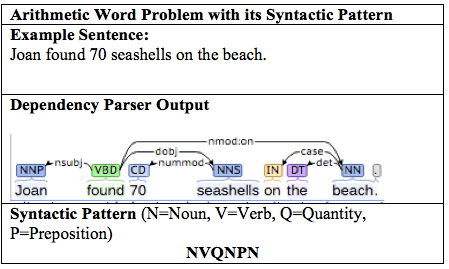
\includegraphics[width=0.6\textwidth]{Figure1}
\centering
\caption{\label{fig:Figure1}Example sentence of a word problem and its syntactic pattern.}
\end{figure}

When taking word problems into consideration, Algebra may be a challenging part from a child's point of view but the semantics of a sentence such as understanding of the syntax, extensive knowledge, coreference resolution, extracting information from individual sentences and combining that information effectively to produce a result is relatively easier. \newline

Our system needs to parse the sentences in a word problem well to fetch useful information. This information needs to be used collectively in an effective way to generate an equation. Solving the equation if generated correctly is a trivial part. Figure 1 shows an example of how a sentence from a word problem is simplified to a syntactic pattern. This paper approaches the problem of solving arithmetic word problems by mapping individual sentences in a word problem to a syntactic pattern. Based on the syntactic pattern each sentence is simplified until it represents minified information which consists of a subject, verb, object with its quantity, preposition if there exists one and other parts of speech. This simplified sentence is then classified to an operator and the quantified noun is added to the equation with the classified operator. Each simplified sentence is classified to one of four operators as described in Table 1.\newline 

We gather information form the sentences by parsing the sentence using the dependency parser \footnote{http://nlp.stanford.edu/software/stanford-dependencies.shtml}. Based on the Part-of-speech tags and relations between the words from the sentence different entities from the sentence are extracted. Expletives, nouns and their quantities, verbs,  conjunctions, adjectives and prepositions are extracted from the sentence and are related to each other based on the relations output by the dependency parser. Based on some rules these extracted entities are used collectively to form a simplified sentence and is provided as an input to the classifier. As explained above the classifier predicts an operator for the simplified sentence. Now that we have the operator we use the operator and the extracted entity in the equation. Consider the below example:
\begin{figure}[h]
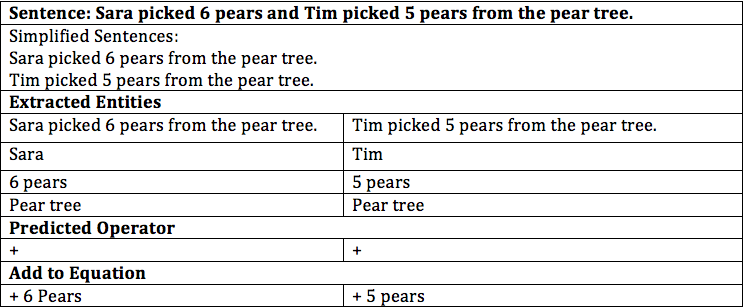
\includegraphics[width=0.90\textwidth]{Figure2}
\centering
\caption{\label{fig:Figure2}Example sentence of a word problem and its simplification.}
\end{figure}

Simplifying the sentences to such format makes it less complex for the classifier to predict an operator corresponding to the sentence as well as it makes things trivial to generate equations. Though the training data seems to be the sentences, actually the sentences in the training data are just a way to generate syntactic patterns which are used extensively as the features to the classifier. A large number of sentences will end up having the same syntactic pattern. Hence, training is actually on syntactic patterns and not on raw text.

Our system learns this classifier based on 300 individual sentences. Our data and source code are publicly available \footnote{Source code and training dataset is available at \url{https://github.com/vishalrajpal/TrySystem}.}. The next section describes how we extract the syntactic pattern, its usage and problem decomposition.


\section{Syntactic Pattern and Problem Decomposition}
\label{method}
In this section we describe how we use the dependency parser output to extract the syntactic pattern of a sentence and the process of simplifying sentences using the extracted syntactic pattern. We further describe the way we predict the operator of the simplified sentence using a Logistic Regression classifier. The input to our system is a problem text and we carry out multiple steps for each sentence in this problem text. Below are the steps:

\subsection{Run Dependency Parser on Each Sentence}
For each sentence in the problem text, we extract the relations and the part-of-speech tags using the dependency parser. Based on the output from the dependency parser we extract the Expletive if any, Nouns and their quantities, preposition, conjunction etc. and build a syntactic pattern based on the ordering of the words in the sentence as described in Figure 1. The representation of a sentence as a syntactic pattern helps us fetch information about this sentence easily such as if the sentence has a quantified noun or a conjunction, an expletive or a preposition etc. We use this information to further simplify the sentence as described in further steps. 

\subsection{Parse Commas in Each Sentence}
In most arithmetic word problems, commas are a way to either multiple subjects interacting with the same object or a subject interacting with multiple objects. Hence, to simplify sentences comma is an important punctuation character. After extracting the syntactic pattern of the overall sentence, the sentence is looked for commas. If any of the commas exist based on some rules we decide if the text before comma belongs to the subject part of the sentence or the object part of the sentence. The goal of this step is to have simplified sentences based on parsing commas in the sentence. The current sentence is replaced by simplified sentences extracted by parsing the sentence based on a comma. Consider the below example:

\begin{figure}[h]
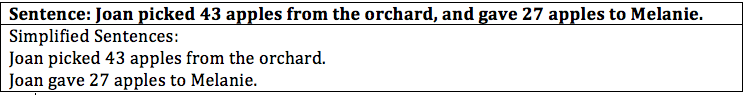
\includegraphics[width=0.90\textwidth]{Figure3}
\centering
\caption{\label{fig:Figure3}Simplification of a sentence based on a comma.}
\end{figure}

\subsection{Run Dependency Parser on Each Sentence}
Now that we have simplified sentences extracted by parsing the sentence based on a comma, we give these simplified sentences to the dependency parser to update the syntactic pattern. The syntactic pattern is extracted in the same way as in Step 2.1. We further apply some rules to extract more simpler sentences.

\subsection{Parse Conjunctions in Each Sentence}
Similar to commas, in most arithmetic problems conjunctions are a way mostly to specify two subjects interacting with a single object, or a single subject interacting with two objects. Based on the updated syntactic pattern from previous step looking if a conjunction exists is trivial. If a conjunction exists we simplify the sentence based on some rules. The goal of this step is to have multiple simplified sentences based on parsing by conjunctions. The current sentence is replaced by simplified sentences extracted by parsing the sentence based on a conjunction. Below is an example where a conjunction "and" exists:

\begin{figure}[h!]
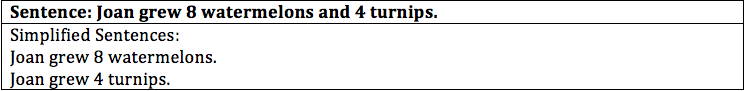
\includegraphics[width=0.90\textwidth]{Figure4}
\centering
\caption{\label{fig:Figure4}Simplification of a sentence based on a conjunction.}
\end{figure}

\subsection{Run Dependency Parser on Each Sentence}
At this point, the sentences are simplified at the most granular level. Since, each sentence is replaced by multiple simplified sentences their will be multiple syntactic patterns. We provide these simplified sentences to the dependency parser and based on the same rules used in the above steps we extract the useful information such as Nouns, verbs etc. Based on the information extracted the features for each sentences are extracted from the syntactic pattern and other properties as described in the next section. At this point, we have a feature vector for a single sentence of the problem text. Each sentence of the problem text will be simplified to multiple sentences and each simplified sentence would have its own feature vector which would be classified to an operator as discussed in the next step.

\subsection{Features} 
\subsubsection{Syntactic Patterns}
All the syntactic patterns extracted from the training data are used as individual features. The syntactic pattern to which the sentence belongs is set and all the other are not in a one-hot encoding way. From the training data of 300 sentences, we extracted near to 125 syntactic patterns, which shows that multiple sentences have a similar syntactic pattern. For test data, even if we haven't seen a pattern before the other features as described below will try to map the syntactic pattern found to the existing syntactic pattern. 

\subsubsection{Count based Features}
Based on our analysis we found that having a count of some important things in the syntactic pattern proves to be helpful to the classifier in learning accurately. There are 4 count based features: number of nouns, number of prepositions, number of verbs and number of quantities. These features depend on how we map the sentence to a syntactic pattern and as explained above if we map the sentence to the correct syntactic pattern, extracting these kind of features is a trivial task.

\subsubsection{Occurrence based Features}
\paragraph{Relation based Occurrence Features}
We use the occurrence of some dependency relations as features. Particularly nmod:poss relation from the dependency parser if set can determine the subject possessing the object and nmod:of which helps to differentiate between two nouns of same kind. The relations in the sentence depict its structure and to simplify the sentences the properties of its structure prove to be helpful.
\paragraph{Pattern based Occurrence Features}
Occurrence of some specific syntactic pattern as a sub pattern of the syntactic pattern of a sentence can also be helpful. We have 2 features: NVQN syntactic pattern and QN syntactic pattern. These two patterns indicate that a sentence of such pattern is mostly suggesting addition or subtraction. Since we are trying to simplify the sentences to a similar pattern, they prove to distinctive features between quantified classes("+", "-") and other classes("=", "?"). 

\paragraph{Word based Occurrence Features}
Some specific words allow the classifier to predict more accurately. The word "now" is suggesting a result after some operation and hence the predicted operator should be "=". Similarly, occurrence of one of the words from "most", "some" and "several" suggests an unknown quantity in the sentence. There are different such words through which we can predict the operation and hence we use the occurrence of such words as features.

\subsubsection{Word similarity based features}
We identified 8 word categories from WordNet and Word2Vec which can be helpful in predicting the operator. The 8 verb categories are "verb.possession", "verb.change", "verb.communication", "verb.consumption" , "verb.contact", "verb.creation", "verb.motion" and "verb.weather". The verbs in the sentence are given as input to WordNet and Word2Vec and the result is normalized between these categories.

\subsection{Training the Classifier to Predict Operator}
At this point we only consider addition and subtraction problems but based on our approach and analysis we believe it is generalizable to multiplication and division problems as well. The possible operators in our system currently are "+", "-", "=" and "?". The "+" operator and "-" are self explanatory, whereas a sentence classified as "=" is suggesting that the quantity in the sentence is a result of some operations and a sentence classified as "?" is suggesting that the sentence is asking a question about some entity.

We train four Logistic Regression binary classifiers for each of the above mentioned operators. We then use one vs all technique to combine the results from these binary classifiers. Our test data contain 55 simplified sentences. The below table consists of the precision and recall for all the 4 classes:

\begin{table}[h]
\begin{center}
\begin{tabular}{|c|c|c|c|}
\hline
\bf Operator & \bf No. of instances & \bf Precision & \bf Recall \\
\hline
+ & 32 & 95.83\% & 71.87\% \\
\hline
- & 9 & 40\% & 66.66\% \\
\hline
= & 2 & 50\% & 50\% \\
\hline
? & 15 & 82.35\% & 93.33\% \\
\hline
\end{tabular}
\end{center}
\caption{\label{precision-recall-table} Precision and Recall}
\end{table}

Based on the results above, it is clear that operator "?" had some specific features such as presence of WH-adverb which made it easy for the classifier to predict question sentences correctly. Preposition occurrence features provided distinctive information to the classifier for operator "+". Operator "-" is entirely dependent on verb features and some preposition occurrence features such as presence of preposition "from". Whereas operator "=" is dependent on some specific word occurrence features such as "now". Below is an example of some sentences classified correctly:

\begin{table}[h]
\begin{center}
\begin{tabular}{|c|c|c|}
\hline
\bf Sentence & \bf Actual Operator & \bf Classified Operator\\
\hline
Sandy has 24 red balloons. & + & +\\
\hline
He took 20 seashells from Joan. & - & -\\
\hline
He now has 21 left. & = & =\\
\hline
How much sugar is remaining? & ? & ?\\
\hline
\end{tabular}
\end{center}
\caption{\label{prediction-example-table} Example Sentences}
\end{table}

%Should we have precision and recall?%

\subsection{Building and Solving Equation}

Based on the operator prediction for a single simplified sentence from the classifier, the quantified noun from sentence is extracted. We assign the label predicted by the classifier for the sentence as explained in the previous step to the quantified noun. When our system encounters a sentence predicted as "?" it extracts the Noun in that sentence and we assume that Noun is the entity for which the computation needs to be done. All the other sentences are looked for similarity with this entity and are merged into an coherent whole equation if they are similar. Once every sentence undergoes this process, we have an equation and computing it is the trivial part. Below is an example of an equation generated by our system:\newline

\begin{table}[h]
\begin{center}
\begin{tabular}{|>{\centering\arraybackslash}m{8cm}|>{\centering\arraybackslash}m{6cm}|}
\hline
\bf Problem Text & \bf Equation Generated by our system\\
\hline
Sandy grew 6 carrots . Sam grew 3 carrots . How many carrots did they grow in total ? & +6 carrots +3 carrots = ? carrots\\
\hline
\end{tabular}
\end{center}
\caption{\label{equation-example-table} Example Problem Text and Equation}
\end{table}

\newpage
\section{Experimental Results}

We evaluate our system on publicly available datasets of arithmetic word problems in this section. In the present state, our system is only able to evaluate addition and subtraction problems. But given the approach we believe that it should not be difficult for the classifier to handle multiplication and division problems. Refer to Section 4.1.

\subsection{Datasets}
We evaluate our system on 3 publicly available datasets from which we only consider the addition and subtraction problems. The evaluation results are mentioned in Table 4. Below is the description of the datasets we have used:

\subsubsection{A12 Dataset}
This dataset consists of 395 addition and subtraction problems, released by ~\cite{Hosseini:14}. They performed a 3-fold cross validation and each fold consists of problems from different sources. We evaluate our system on this dataset with the same settings and report our results.

\subsubsection{IL Dataset}
This dataset is a collection of arithmetic problems released by ~\cite{Roy:15}. We extract all the addition and subtraction problems. Each problem in this dataset has a single operation involved.

\subsubsection{Commoncore Dataset}
This dataset is a collection of 600 multistep problems released by ~\cite{Roy:15}. There are 6 types of problems with 100 problems for each type. We consider 100 problems of type "Addition followed by Subtraction".\newline

\begin{table}[h]
\begin{center}
\begin{tabular}{|c|c|c|c|}
\hline
\bf & \bf A12 & \bf IL & \bf CC \\
\hline
 & 60\% & 72.88\% & 50\% \\
\hline
~\cite{Roy:15} & 78\% & 73.9\% & 45.2\% \\
\hline
~\cite{Kushman:15} & 64\% & 73.7\% & 2.3\% \\
\hline
~\cite{Hosseini:14} & 77.7\% & - & - \\
\hline
~\cite{Roy: 15} & - & 52.7 & - \\
\hline
\end{tabular}
\end{center}
\caption{\label{results-table} Accuracy in correctly solving arithmetic problems.}
\end{table}

The first row in the above table represents the accuracy for our system. We achieve an improvement in the multi step common core dataset released by ~\cite{Roy:15}. For the IL dataset we have competitive results. The important point to notice is that majority of the errors are classification errors as described in Section 4.2.

\section{Discussion}
The approach our system follows is generalized in a way that it gives importance to every Part of Speech in a sentence. Not only verbs but other Parts of Speech such as preposition play an important role while solving arithmetic word problems. Our system learns to simplify the sentences which makes it easy for the classifier to predict an operator for that sentence. 

\subsection{Future Work}

\subsubsection{Multiplication and Division Problems}
In this paper, we have focused on addition and subtraction problems, we aim to deal with multiplication and division problems. Based on our analysis of the approach, we believe that by adding some additional features and training data, multiplication and division problems could be solved.
\newpage
\subsubsection{Additional Complex Parsing Rules}
Our system currently employs simple rules but is able to solve arithmetic problems efficiently. Though our system shows improvement in parsing as compared to ~\cite{Hosseini:14}, we aim to focus on adding more complex rules to extract quantified nouns. Sentences in some of the problems were classified correctly, but the extraction of quantified nouns wasn't accurate. We look to improve this in future.

\subsubsection{Improving the Classifier}
We also plan to focus on improving our classifier through some advanced methods. At this point, we have a Logistic Regression classifier which performs reasonably well. This might be an area to predict the operator more accurately. We plan to consider Ensembling in future to predict the operator for simplified sentences.

\subsection{Detailed Error Analysis}
\begin{table}[h]
\begin{center}
\begin{tabular}{|>{\centering\arraybackslash}m{8cm}|>{\centering\arraybackslash}m{6cm}|}
\hline
\bf Error Type & \bf Example \\
\hline
Classification Errors (75\%) & He now has 56 books in his library. \textbf{Classified to "+" but should be "="}. \\
\hline
Parsing Issues (15\%) & Sara has 31 \textbf{red} and 15 green balloons. \\
\hline
Coreference Resolution (10\%) & When they cleaned them , they discovered that \textbf{29} were cracked. \\
\hline
\end{tabular}
\caption{\label{error-analysis-table} Examples of different error categories and relative frequencies.}
\end{center}
\end{table}

\section{Conclusion}
We present an approach to understand and solve general arithmetic problems which used sentence simplification at its core. Our system learns to predict an operator corresponding to each simplified sentence using syntactic patterns, part-of-speech features and occurrence features..The training data to the classifier are simple sentences which have a single quantified noun. Our system extracts the quantified nouns, takes other properties of the sentence into consideration and predicts an operator. The quantified noun is associated with that operator and used in the equation. This also provides ways to discard irrelevant information. The core idea of our approach is to use the basic properties of the language and simplify the task of for the classifier to predict the operator for the sentences.\newline
Though we have simplified sentences in our training data, actually the syntactic patterns of those sentences are used to train the classifier with some limited word occurrence features. We were able to notice an improvement in parsing errors which is a prerequisite to sentence simplification.  Also, our approach generalizes to data from different domains in a better way as we only depend on the syntactic pattern of the sentence and some other properties.\newline

\newpage

\begin{thebibliography}{}
  
  \bibitem[\protect\citename{Korhonen, Anna}2002]{Anna:02}
  Anna Korhonen
  \newblock Assigning Verbs to Semantic Classes via WordNet
  \newblock 2002.
  \newblock {\em Association for Computational Linguistics}
  
  \bibitem[\protect\citename{M�rquez \bgroup et al. \egroup}2015]{M�rquez:15}
  Llu�s M�rquez, Chris Callison-Burch, Jian Su, Daniele Pighin and Yuval Marton
  \newblock Solving Geometry Problems: Combining Text and Diagram Interpretation
  \newblock 2015.
  \newblock {\em The Association for Computational Linguistics}

  \bibitem[\protect\citename{M�rquez \bgroup et al. \egroup}2015]{M�rquez:15}
  Llu�s M�rquez, Chris Callison-Burch, Jian Su, Daniele Pighin and Yuval Marton
  \newblock Automatically Solving Number Word Problems by Semantic Parsing and Reasoning
  \newblock 2015.
  \newblock {\em The Association for Computational Linguistics}
  
  \bibitem[\protect\citename{M�rquez \bgroup et al. \egroup}2015]{M�rquez:15}
  Llu�s M�rquez, Chris Callison-Burch, Jian Su, Daniele Pighin and Yuval Marton
  \newblock Learn to Solve Algebra Word Problems Using Quadratic Programming
  \newblock 2015.
  \newblock {\em The Association for Computational Linguistics}

  \bibitem[Corro and Gemulla]{Corro:13}
  Luciano Del Corro and Rainer Gemulla. 2013. 
  \newblock ClausIE: clause-based open information extraction. 
  \newblock In Proceedings of the 22nd international conference on World Wide Web (WWW '13). ACM, New York, NY, USA, 355-366.
  
  \bibitem[\protect\citename{Hosseini \bgroup et al.\egroup}2014]{Hosseini:14}
  Mohammad Javed Hosseini, Hannaneh Hajishirzi, Oren Etzioni and Nate Kushman.
  \newblock Learning to Solve Arithmetic Word Problems with Verb Categorization
  \newblock 2014.
  \newblock {\em In Proceedings of the EMNLP}

  \bibitem[\protect\citename{Clark \bgroup et al. \egroup}2016]{Clark:16}
  Peter Clark, Oren Etzioni, Tushar Khot, Ashish Sabharwal, Oyvind Tafjord, Peter D. Turney and Daniel Khashabi
  \newblock Combining Retrieval, Statistics, and Inference to Answer Elementary Science Questions
  \newblock 2016.
  \newblock {\em Proceedings of the Thirtieth {AAAI} Conference on Artificial Intelligence, February 12-17, 2016, Phoenix, Arizona, {USA.}}
  
  \bibitem[\protect\citename{Rik \bgroup et al. \egroup}2015]{Rik:15}
  Rik Koncel-Kedziorski , Hannaneh Hajishirzi, Ashish Sabharwal, Oren Etzioni and Siena Ang
  \newblock Parsing Algebraic Word Problems into Equations
  \newblock 2015.
  \newblock {\em Transactions of the Association for Computational Linguistics}

 \bibitem[\protect\citename{Roy and Roth}2015]{Roy:15}
  Subhro Roy and Dan Roth
  \newblock Solving General Arithmetic Word Problems
  \newblock 2015.
  \newblock {\em The Association for Computational Linguistics}
  
  \bibitem[\protect\citename{Roy \bgroup et al. \egroup}2015]{Roy:15}
  Subhro Roy, Tim Vieira and Dan Roth
  \newblock Reasoning about Quantities in Natural Language
  \newblock 2015.
  \newblock {\em Transactions of the Association for Computational Linguistics}
    
  \bibitem[\protect\citename{Mikolov \bgroup et al. \egroup}2013]{Mikolov:13}
  Tomas Mikolov, Kai Chen, Greg Corrado and Jeffrey Dean
  \newblock Efficient Estimation of Word Representations in Vector Space
  \newblock 2013.
  \newblock {\em CoRR}
  
\end{thebibliography}

\end{document}